This section presents our progress towards performing valve turning task set by the DARPA Robotics Challenge (DRC) Event \#7\cite{drc}. 
The task requires that a robot locate, approach, grasp, and turn an industrial valve with two hands.
A core constraint for the DRC is that communications with the robot are limited, making conventional tele-operation is infeasible.
Thus, the valve-turning task requires a straightforward way for a user to command the robot to perform complex actions. 

\begin{figure}[thpb]
  \centering

      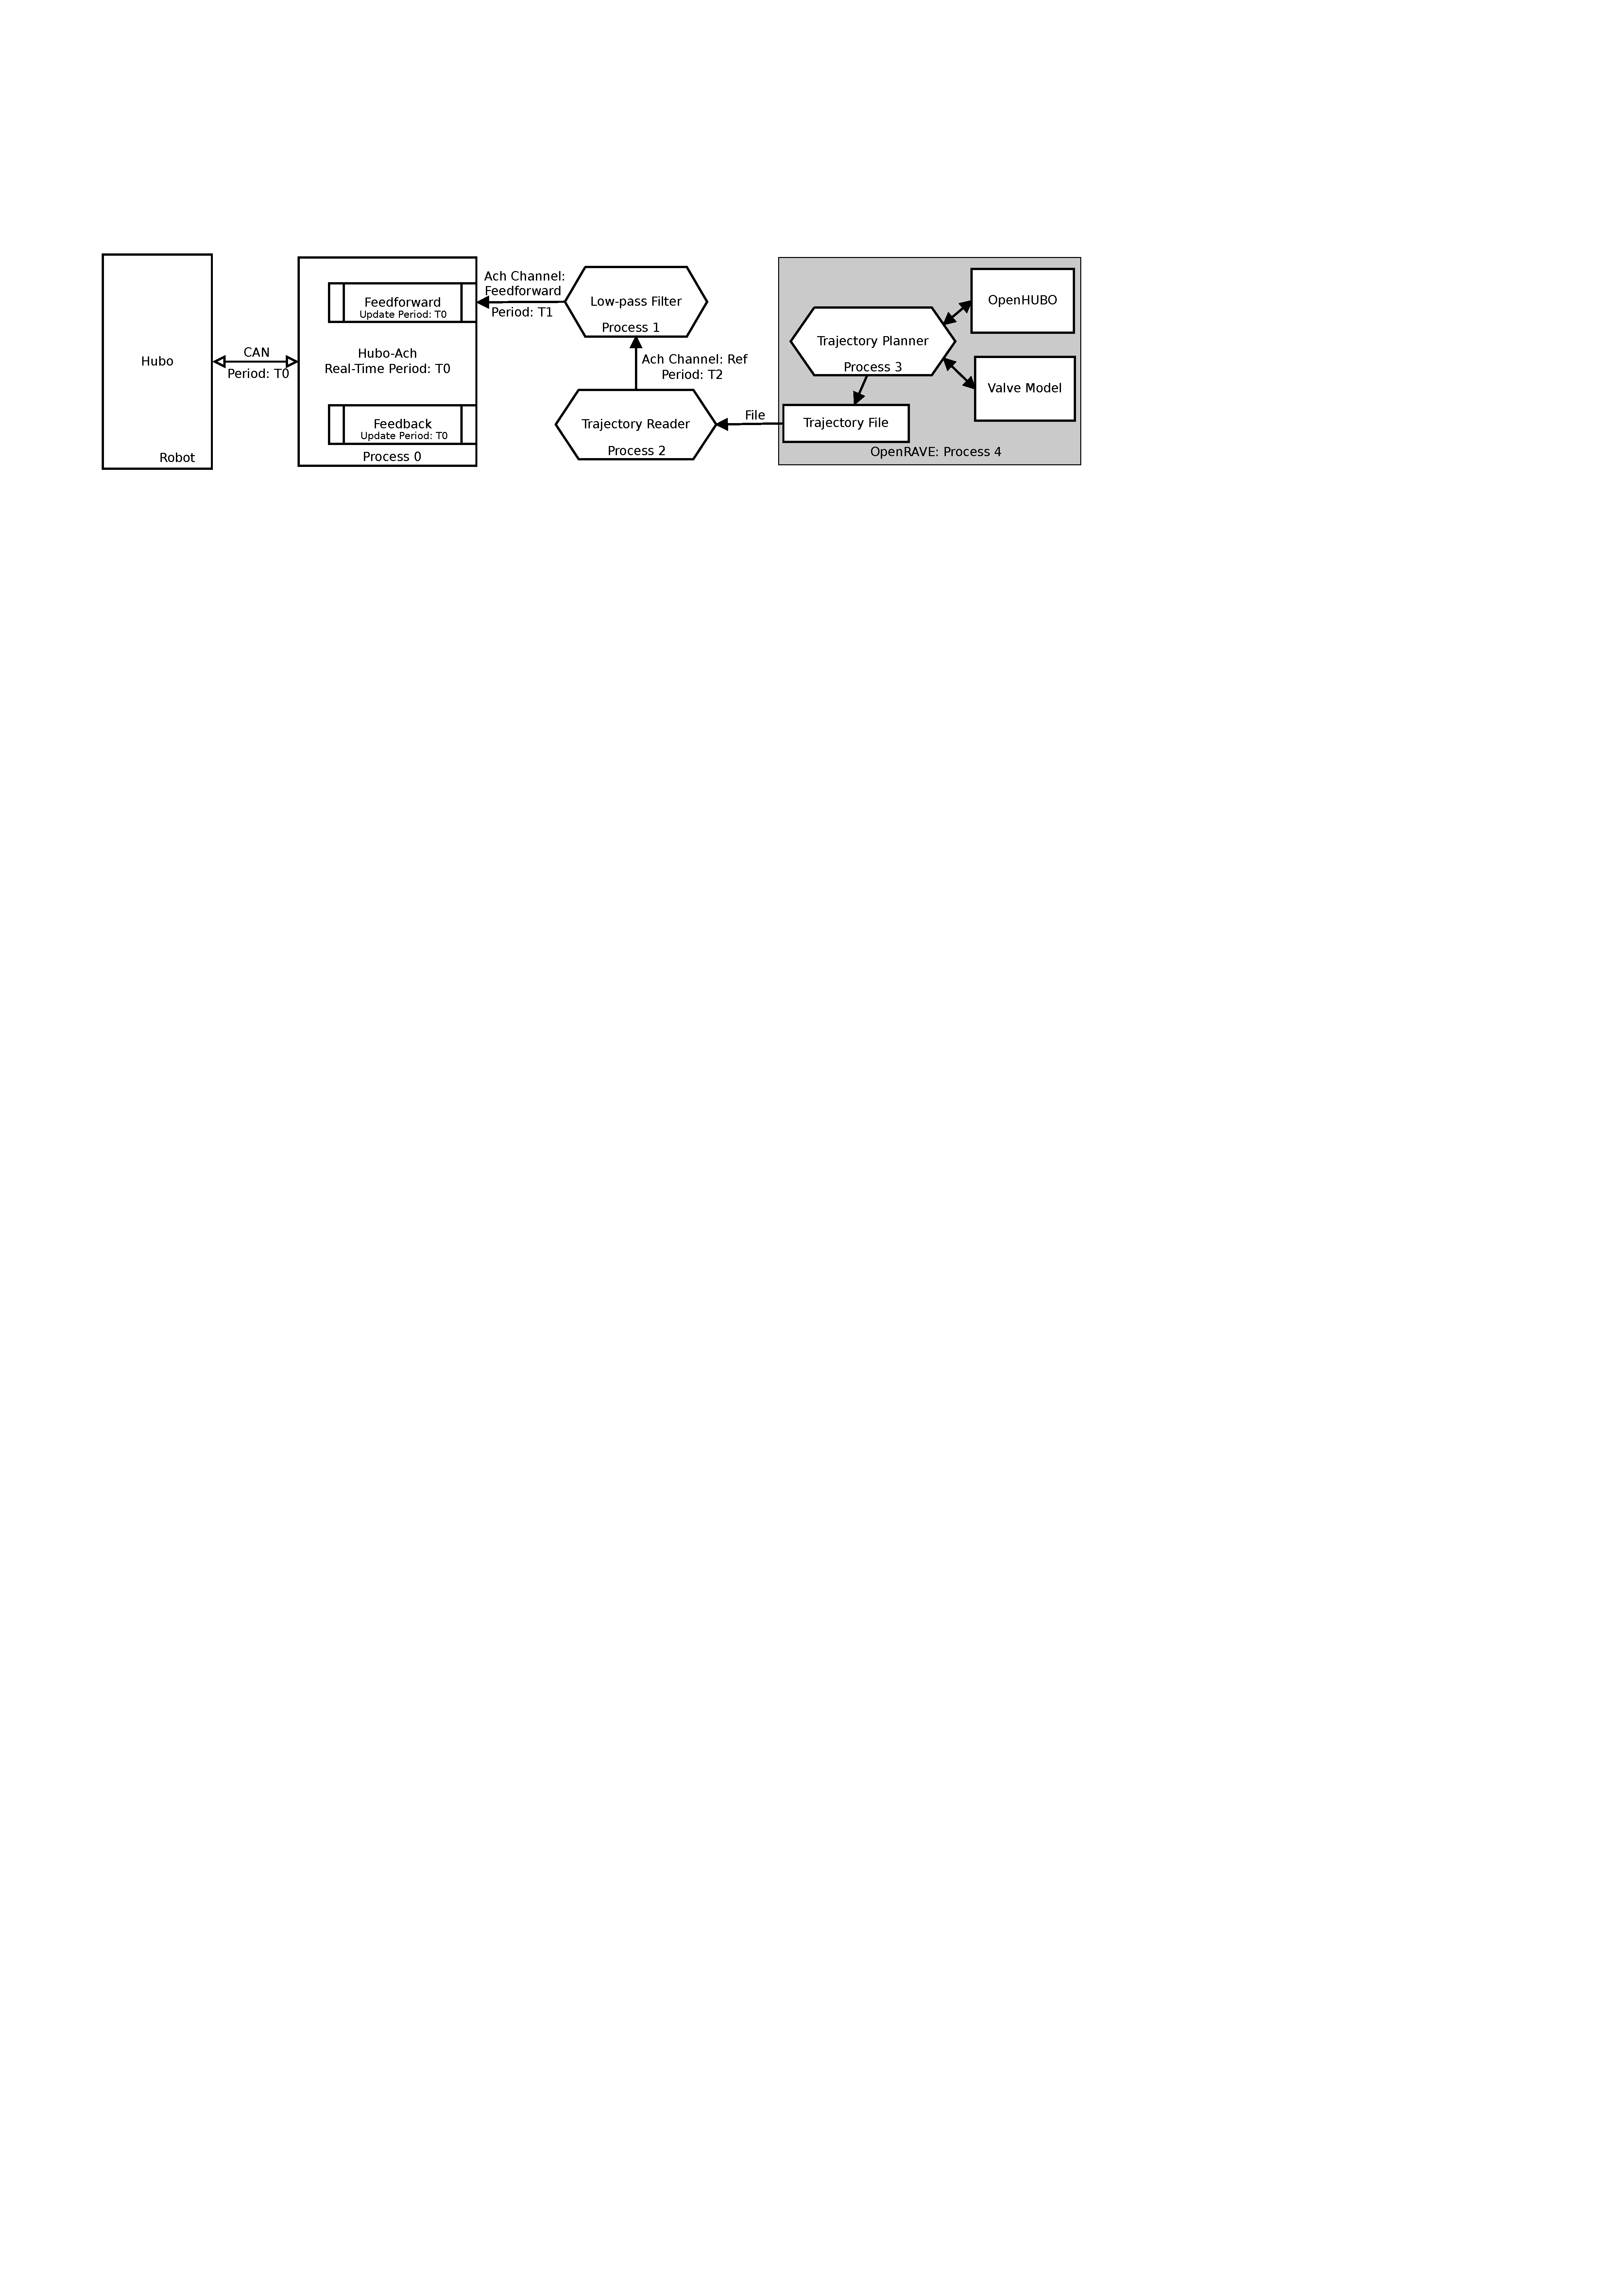
\includegraphics[width=1.0\columnwidth]{./examples/pix/hubo-ach-diagram-openhubo-valve.pdf}

\caption{Block diagram of Hubo-Ach being used for the DRC event \#7, valve turning.  
The process to get the Hubo to turn a valve consists of loading a model of the Hubo and the valve into the simulator.  
OpenRAVE is used as the simulator using the OpenHubo model of Hubo.  
The trajectory planner uses CBiRRT to plan a collision free statically stable joint space path.  
Once the planning is completed the resulting joint space trajectory it is sent through a low-pass filter then sent to the Hubo.}
  \label{fig:block-valve}
\end{figure}



Fig.~\ref{fig:block-valve} shows the block diagram of Hubo-Ach being used for the DRC event \#7, valve turning.  
The process to get the Hubo to turn a valve consists of loading a model of the Hubo and the valve into the simulator.  
OpenRAVE is used as the simulator using the OpenHubo model of Hubo.  
The trajectory planner uses CBiRRT to plan a collision free statically stable joint space path.  
Once the planning is completed the resulting joint space trajectory it is sent through a low-pass filter then sent to the Hubo.
Fig.~\ref{fig:valve} shows the Hubo turning a valve using this method.








\subsection{Planning}
The planning package plans trajectories for high degree of freedom robots so that they can perform object manipulation.
The initial configuration of the robot is critical to manipulation because the robot must be able to:
\begin{itemize}
\item reach and manipulate the object for the entirety of the desired trajectory,
\item maintain balance during execution,
\item avoid self-collisions and collisions with the environment
\end{itemize}
Motion planning is provided by the Constrained Bi-Directional Rapidly-exploring Random Tree (CBiRRT), an efficient and probabilistically complete manipulation planning suite. 
CBiRRT consists of three main components: constraint
representation, constraint-satisfaction, and a general planning algorithm. 
For full details of CBiRRT and its implementation, see Berenson et. al.\cite{Berenson_2011_6867}.

\subsection{Experiment}
Our preliminary experiments with the Hubo were centered around validating our method of motion planning for the robot and evaluating the robot’s capabilities in relation to the requirements of our DRC task (turning the valve). 
These tests were performed on the Hubo2+ at MIT and Drexel University, housed in the lab of Professor Russ Tedrake and Paul Oh respectively.
Our experiments confirmed that the planning system enabled control of the Hubo and that the Hubo was physically capable of turning the valve.
A full description of our methods and experiment can be found in \cite{lofaroTePRA2013Valve}.









\begin{figure}[thpb]
  \centering
  %\begin{tikzpicture}
    %\clip [rounded corners=1em] (0,0) rectangle coordinate (centerpoint) (5,7.5cm);
%    \node[minimum width=\linewidth,minimum height=174pt,draw=black,rounded corners=1em,fill=bgcolor,draw=black]
%    {};
%    \node[name=img] {
      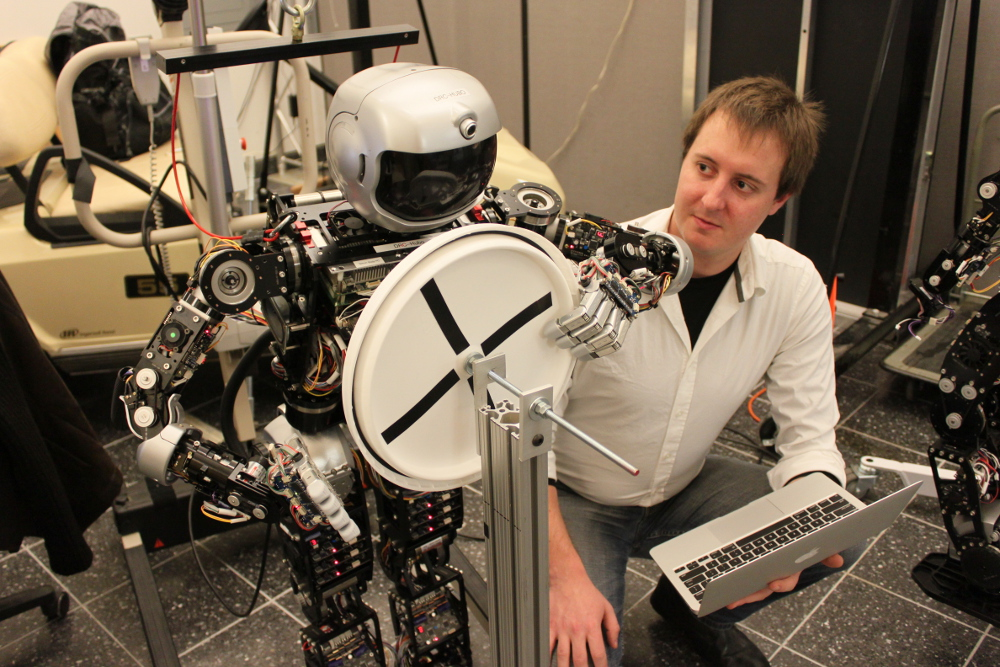
\includegraphics[width=0.69\columnwidth]{./pix/IMG_9107-small.jpg}
      
\includegraphics[width=0.3\columnwidth]{./qrcode/qrcode-valve.png}\\
      Video: http://danlofaro.com/phd/valve/
%    };
%    \draw [bgcolor, rounded corners=1em, line width=1em,inner sep=0pt]
%    (img.north west) --
%    (img.north east) --
%    (img.south east) --
%    (img.south west) -- cycle
%    ;
%  \end{tikzpicture}
\caption{Hubo (left) turning a valve via Hubo-Ach alongside Daniel
  M. Lofaro (right).  Valve turning developed in conjunction with
  Dmitry Berenson at WPI for the DARPA Robotics Challenge.}
  \label{fig:valve}
\end{figure}
